\documentclass[a4paper, 12pt]{article}

\usepackage{utils}

\renewcommand*{\today}{03 septembre 2025}

\begin{document}

\hotbox{Fonction à plusieurs variables}{CM 1}{\today}

\section{Espaces vectoriels normés}

\vspace{5mm}

\begin{definition}
    Étant donné un $\K$-ev $E$, on appelle \textbf{norme} sur $E$ toute application
    $\funcdef{\|.\|}{E}{\R_+}{v}{\|v\|}$ vérifiant les trois propriétés suivantes:
    \begin{itemize}
        \item \textbf{homogénéité:} $\forall(\lambda, x) \in \K \times E, \|\lambda x\| = |\lambda|\|x\|$
        \item \textbf{séparation:} $\forall x \in E, \|x\| = 0 \implies x = 0$
        \item \textbf{inégalité triangulaire:} $\forall(x, y) \in E^2, \|x + y\| \leq \|x\| + \|y\|$
    \end{itemize}
\end{definition}

\begin{definition}
    Un espace vectoriel muni d'une norme est appelé \textbf{espace vectoriel normé} (abrégé par evn ou e.v.n).
\end{definition}

\noindent
Dans ce chapitre, $\K$ désigne un corps et $E$ et $F$ sont deux $\K$-espace vectoriels normés.

\begin{exemple}
    \n
    \begin{enumerate}
        \item La valeur absolue $|.|$ sur $\R$
        \item Le module $|.|$ pour l'espace vectoriel $\C$
        \item Pour $n \in \N$ la norme $\ell^1$ sur $\R^n$ définie par:
        $$
        \forall x = (x_1, \ldots, x_n) \in \R^n, \|x\|_1 = \sum_{i=1}^n |x_i|
        $$
        \item Pour $n \in \N$ la norme $\ell^2$ sur $\R^n$ définie par:
        $$
        \forall x = (x_1, \ldots, x_n) \in \R^n, \|x\|_2 = \sqrt{\sum_{i=1}^n x_i^2}
        $$
        \item Pour $n \in \N$ la norme $\ell^\infty$ sur $\R^n$ définie par:
        $$
        \forall x = (x_1, \ldots, x_n) \in \R^n, \|x\|_\infty = \max(|x_1|, \ldots, |x_n|)
        $$
    \end{enumerate}
\end{exemple}

\begin{definition}
    Pour $x = (x_i)_{1\leq i \leq n}, y = (y_i)_{1\leq i \leq n} \in \R^n$, le produit scalaire est usuellement définit par:
    $$
    \langle x, y \rangle = \sum_{i=1}^n x_i y_i
    $$
    noté aussi $(x | y)$ ou même $\langle x | y \rangle$
\end{definition}

\begin{remarque}
    On a $||x||_2 = \sqrt{\langle x, x \rangle}$
\end{remarque}

\begin{lemme}{Inégalité de Cauchy-Schwarz}{}
    $\forall x, y \in \R^n, |\langle x, y \rangle| \leq ||x||_2 ||y||_2$
    avec égalité si et seulement si $x$ et $y$ sont colinéaires.
\end{lemme}

\begin{demonstration}
    Soient $x, y \in \R^n$.\n
    On pose le polynôme $P(t) := \langle x + ty, x + ty \rangle$.
    \begin{align*}
        P(t) &= \|x+ty\|\\
        &= \sum_{i=1}^n (x_i + ty_i)^2\\
        &= \sum_{i=1}^n (x_i^2 + 2tx_iy_i + t^2y_i^2)\\
        &= t^2 \sum_{i=1}^n y_i^2 + 2t \sum_{i=1}^n x_iy_i + \sum_{i=1}^n x_i^2\\
        &= t^2 \langle y, y \rangle + 2t \langle x, y \rangle + \langle x, x \rangle\\
    \end{align*}
    D'une part comme $P(t) = ||x + ty||^2 \geq 0$, le discriminant de $P$ est négatif ou nul:
    \begin{align*}
        \Delta = 4\langle x, y \rangle^2 - 4\langle y, y \rangle \langle x, x \rangle &\leq 0\\
        \implies \langle x, y \rangle^2 &\leq \langle y, y \rangle \langle x, x \rangle\\
        \implies |\langle x, y \rangle| &\leq \sqrt{\langle y, y \rangle} \sqrt{\langle x, x \rangle}\\
        \implies |\langle x, y \rangle| &\leq ||x||_2 ||y||_2
    \end{align*}
    D'autre part quand $P(t)$ admet une racine double, on a $t_0 = -\frac{\langle x, y \rangle}{\langle y, y \rangle}$ et $P(t_0) = \|x + t_0y\|^2 = 0 \implies x + t_0y = 0 \implies x = -t_0y$
    avec $t_0 = -\frac{\langle x, y \rangle}{\langle y, y \rangle}$ d'où $x$ et $y$ colinéaires en cas d'égalité.
\end{demonstration}

\begin{proposition}{}{}
    La norme euclidienne $||.||_2$ est bien une norme.\n
    De plus $||x + y|| = ||x|| + ||y||$ si et seulement si $x$ et $y$ sont colinéaires et de même sens.
\end{proposition}

\begin{demonstration}[Norme euclidienne $\ell^2$]
    Soient $x = (x_i)_{1\leq i \leq n}, y = (y_i)_{1\leq i \leq n} \in \R^n$.

    \begin{enumerate}
        \item (Homogénéité)
        Soit $\lambda \in \R$, 
        \begin{align*}
            ||\lambda x ||_2 &= \sqrt{\sum_{i=1}^n (\lambda x_i)^2}\\
            &= \sqrt{\lambda^2 \sum_{i=1}^n x_i^2}\\
            &= |\lambda| \sqrt{\sum_{i=1}^n x_i^2}\\
            &= |\lambda| ||x||_2
        \end{align*}
        \item (Séparation)\n
        La contraposée de la séparation est: $\forall x \in \R^n, x \neq 0 \implies \|x\|_2 \neq 0$.\n
        Soit $x \in \R^n, x \neq 0$, ainsi $\exists i \in \llbracket 1, n \rrbracket$ tel que $x_i \neq 0$.\n
        Donc $||x||_2 \geq \sqrt{x_i^2} = |x_i| \gt 0$.
        \item (Inégalité triangulaire)\n
        On utilise l'inégalité de Cauchy-Schwarz $\textcolor{red}{|\langle x,y \rangle|} \leq \textcolor{blue}{\|x\|_2\|y\|_2}$.\n
        \begin{align*}
            \|x + y\|_2^2 &= \sqrt{\sum_{i=1}^n (x_i + y_i)^2}\\
            &= \sqrt{\sum_{i=1}^n (x_i^2 + 2x_iy_i + y_i^2)}\\
            &=\sqrt{\sum_{i=1}^n x_i^2 + 2\sum_{i=1}^n x_iy_i + \sum_{i=1}^n y_i^2}\\
            &=\sqrt{\sum_{i=1}^n x_i^2} + 2\sqrt{\sum_{i=1}^n x_iy_i} + \sqrt{\sum_{i=1}^n y_i^2}\\
            &= \|x\|_2^2 + 2\textcolor{red}{\langle x, y \rangle} + \|y\|_2^2\\
            &\leq \|x\|_2^2 + 2\textcolor{blue}{\|x\|_2\|y\|_2} + \|y\|_2^2\\
            &= (\|x\|_2 + \|y\|_2)^2\\
            \implies \|x + y\|_2 &\leq \|x\|_2 + \|y\|_2
        \end{align*}
    \end{enumerate}
\end{demonstration}

\begin{demonstration}[cas d'égalité dans l'inégalité triangulaire]
    si $x$ et $y$ sont colinéaires avec le cas de l'égalité de Cauchy-Schwarz
        on a:
        \begin{itemize}
            \item si $\langle x, y\rangle \geq 0$ alors $||x + y||_2^2 = \|x\|_2^2 + 2|\langle x, y \rangle| + \|y\|_2^2 \leq (\|x\|_2 + \|y\|_2)^2$
            \item si $\langle x, y \rangle \lt 0$ alors $||x + y||_2^2 = \|x\|_2^2 - 2|\langle x, y \rangle| + \|y\|_2^2 \leq \|x\|_2^2 - 2\|x\|_2\|y\|_2 + \|y\|_2^2 = (\|x\|_2 - \|y\|_2)^2 \leq (\|x\|_2 + \|y\|_2)^2$
        \end{itemize}
        \begin{hotwarn}
            à retravailler car pas très clair
        \end{hotwarn}
\end{demonstration}

\begin{proposition}{Seconde inégalité triangulaire}{}
    Soit $(E, \|.\|)$ un evn, $soient x, y \in E$.
    $$
    \forall x, y \in E, \|x - y\| \geq |\|x\| - \|y\||
    $$
    avec égalité si et seulement si $x$ et $y$ sont colinéaires.
\end{proposition}

\begin{demonstration}
    Soient $x, y \in E$
    
    \begin{align*}
        \|x\| &= \|x - y + y\|\\
        &\leq \|x - y\| + \|y\|\\
        \implies \|x\| - \|y\| &\leq \|x - y\|
    \end{align*}
    en échangeant $x$ et $y$, on obtient $\|y\| - \|x\| \leq \|y - x\| = \|x - y\|$
    \n
    d'où $|\|x\| - \|y\|| \leq \|x - y\|$
    avec égalité si et seulement si $x$ et $y$ sont colinéaires.
\end{demonstration}

\begin{methode}
    On peut conclure sur une inégalité triangulaire générale
    
    $|\|x - y\|| \leq \| x \pm y\| \leq \|x\| + \|y\|$
    pour tous $x, y \in E$.
\end{methode}

\section{Les boules}

\vspace{5mm}

\begin{definition}[(Boule ouverte)]
    On appelle \textbf{boule ouverte} de centre $a$ et de rayon $r$ l'ensemble:
    $$
    B(a, r) = \{x \in E \mid \|x - a\| \lt r\}
    $$
\end{definition}
\begin{definition}[(Boule fermée)]
    On appelle \textbf{boule fermée} de centre $a$ et de rayon $r$ l'ensemble:
    $$
    \overline{B}(a, r) = \{x \in E \mid \|x - a\| \leq r\}
    $$
    peut aussi se noter $B_f(a, r)$
\end{definition}
\begin{definition}[(Sphère)]
    On appelle \textbf{sphère} de centre $a$ et de rayon $r$ l'ensemble:
    $$
    S(a, r) = \{x \in E \mid \|x - a\| = r\}
    $$
\end{definition}

\begin{remarque}
    Lorsque qu'on travaille en dimension 2, on parle de \textbf{disque ouvert/fermé}.
    Ainsi on peut retrouver $D(a, r)$ et $\overline{D}(a, r)$ pour les boules ouvertes et fermées respectivement.
\end{remarque}

\begin{figure}[h]
    \centering
    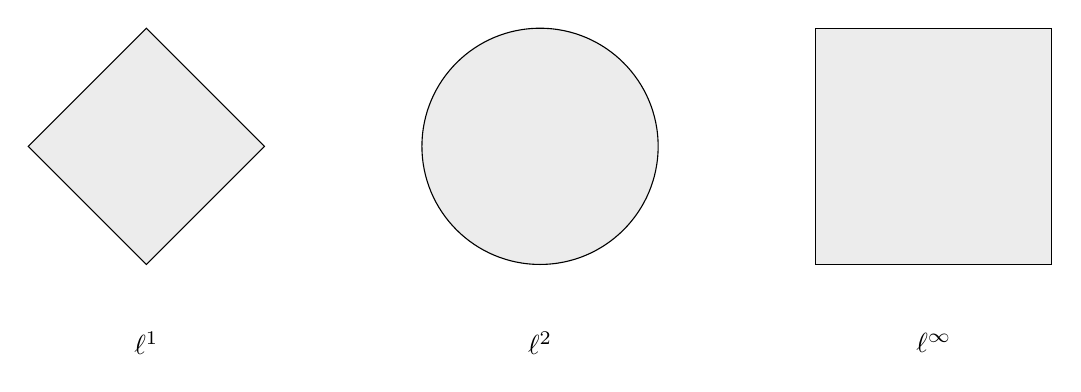
\begin{tikzpicture}[scale=1]
        \begin{scope}
            \fill[gray!15] (0,1.5)--(1.5,0)--(0,-1.5)--(-1.5,0)--cycle;
            \draw[thin] (0,1.5)--(1.5,0)--(0,-1.5)--(-1.5,0)--cycle;
            \ballGraph
            \node at (0,-2.5) {$\ell^1$};
        \end{scope}
        \begin{scope}[xshift=5cm]
            \fill[gray!15] (0,0) circle(1.5);
            \draw[thin] (0,0) circle(1.5);
            \ballGraph
            \node at (0,-2.5) {$\ell^2$};
        \end{scope}
        \begin{scope}[xshift=10cm]
            \fill[gray!15] (-1.5,-1.5) rectangle (1.5,1.5);
            \draw[thin] (-1.5,-1.5) rectangle (1.5,1.5);
            \ballGraph
            \node at (0,-2.5) {$\ell^\infty$};
        \end{scope}
    \end{tikzpicture}
    \caption{Boules pour les normes $\ell^1, \ell^2$ et $\ell^\infty$ sur $\R^2$}
    \label{fig:boules}
\end{figure}

\begin{definition}
    Soit $\xn{x} \in E^\N$ une suite.\n
    On dit que $(x_n)$ converge vers $l \in E$ si
    $$
    \lim \|x_n - l\| = 0
    $$
\end{definition}

\begin{remarque}
    On y voit une meilleure interprétation quand on sait que $\|x_n - l\|$ est la distance entre $x_n$ et $l$.
\end{remarque}

\begin{definition}[(intérieur)]
    Soit $A \subset E$.\n
    On dit que $a \in A$ est \textbf{intérieur} à $A$ si 
    $$
    \exists r \gt 0,\, B(a, r) \subset A
    $$
    \textbf{L'intérieur} de $A$ est l'ensemble des points intérieurs de $A$ et on le note $\text{int}(A)$ ou encore $\mathring{A}$.\n
    On dit que $A$ est un \textbf{ouvert} si $A = \mathring{A}$.
\end{definition}

\begin{definition}[(adhérence)]
    Soit $A \subset E$.\n
    On dit que $a \in E$ est \textbf{adhérent} à $A$ si 
    $$
    \forall r \gt 0,\, B(a, r) \cap A \neq \emptyset
    $$
    \textbf{L'adhérence} de $A$ est l'ensemble des points adhérents de $A$ et on le note $\text{adh}(A)$ ou encore $\overline{A}$.\n
    On dit que $A$ est un \textbf{fermé} si $A = \overline{A}$.
\end{definition}

\begin{definition}[(Frontière)]
    Soit $A \subset E$.\n
    On appelle \textbf{frontière} de $A$ l'ensemble:
    $$
    \partial A = \overline{A} \setminus \mathring{A}
    $$
\end{definition}

\begin{proposition}{}{}
    Soit $A \subset E$
    $$
    A = \mathring{A} = \overline{A} \implies A = E \text{ ou } A = \emptyset
    $$
\end{proposition}

\begin{hotwarn}
    Démonstration à faire
\end{hotwarn}

\end{document}
